%%%%%%%%%%%%%%%%%%%%%%% file template.tex %%%%%%%%%%%%%%%%%%%%%%%%%
%
% This is a general template file for the LaTeX package SVJour3
% for Springer journals.          Springer Heidelberg 2010/09/16
%
% Copy it to a new file with a new name and use it as the basis
% for your article. Delete % signs as needed.
%
% This template includes a few options for different layouts and
% content for various journals. Please consult a previous issue of
% your journal as needed.
%
%%%%%%%%%%%%%%%%%%%%%%%%%%%%%%%%%%%%%%%%%%%%%%%%%%%%%%%%%%%%%%%%%%%
%
% First comes an example EPS file -- just ignore it and
% proceed on the \documentclass line
% your LaTeX will extract the file if required
\begin{filecontents*}{example.eps}
%!PS-Adobe-3.0 EPSF-3.0
%%BoundingBox: 19 19 221 221
%%CreationDate: Mon Sep 29 1997
%%Creator: programmed by hand (JK)
%%EndComments
gsave
newpath
  20 20 moveto
  20 220 lineto
  220 220 lineto
  220 20 lineto
closepath
2 setlinewidth
gsave
  .4 setgray fill
grestore
stroke
grestore
\end{filecontents*}
%
\RequirePackage{fix-cm}
%
%\documentclass{svjour3}                     % onecolumn (standard format)
%\documentclass[smallcondensed]{svjour3}     % onecolumn (ditto)
\documentclass[smallextended]{svjour3}       % onecolumn (second format)
%\documentclass[twocolumn]{svjour3}          % twocolumn
%
\smartqed  % flush right qed marks, e.g. at end of proof
%
\usepackage{graphicx}
\usepackage{amsmath, amssymb}
\usepackage{amsfonts}
\usepackage{caption}
\usepackage{subcaption}
\usepackage{hyperref}
\usepackage{pdflscape}
\usepackage{color}
\usepackage{enumerate}
\usepackage{enumitem}
\usepackage{mathtools}

\renewcommand{\labelitemi}{$\bullet$}
\captionsetup{compatibility=false}

\newtheorem{prop}{Proposition}

%
% \usepackage{mathptmx}      % use Times fonts if available on your TeX system
%
% insert here the call for the packages your document requires
%\usepackage{latexsym}
% etc.
%
% please place your own definitions here and don't use \def but
% \newcommand{}{} 
%
% Insert the name of "your journal" with
% \journalname{myjournal}
%



% original amsmath definition
% \subequations:
% \long macro:->\refstepcounter {equation}\protected@edef \theparentequation {\theequation }\setcounter {parentequation}{\value {equation}}\setcounter {equation}{0}\def \theequation {\theparentequation \alph {equation}}\ignorespaces 

% saved by hyperref in
% > \HyOrg@subequations=\long macro:

% hyperref-patched \subequations: (\endsubequations not modified)
% > \subequations=macro:
% ->\stepcounter {equation}\protected@edef \theHparentequation {\@ifundefined {th
% eHequation}\theequation \theHequation }\addtocounter {equation}{-1}\HyOrg@subeq
% uations \def \theHequation {\theHparentequation \alph {equation}}\ignorespaces 
% .


% extending the environment
%   1. with optional parameter: expected values resume or intermezzo or none.
%   2. while keeping the hyperref customization.

\makeatletter
\def\user@resume{resume}
\def\user@intermezzo{intermezzo}
%
\newcounter{previousequation}
\newcounter{lastsubequation}
\newcounter{savedparentequation}
\setcounter{savedparentequation}{1}
% 
\renewenvironment{subequations}[1][]{%
      \def\user@decides{#1}%
      \setcounter{previousequation}{\value{equation}}%
      \ifx\user@decides\user@resume 
           \setcounter{equation}{\value{savedparentequation}}%
      \else  
      \ifx\user@decides\user@intermezzo
           \refstepcounter{equation}%
      \else
           \setcounter{lastsubequation}{0}%
           \refstepcounter{equation}%
      \fi\fi
      \protected@edef\theHparentequation{%
          \@ifundefined {theHequation}\theequation \theHequation}%
      \protected@edef\theparentequation{\theequation}%
      \setcounter{parentequation}{\value{equation}}%
      \ifx\user@decides\user@resume 
           \setcounter{equation}{\value{lastsubequation}}%
         \else
           \setcounter{equation}{0}%
      \fi
      \def\theequation  {\theparentequation  \alph{equation}}%
      \def\theHequation {\theHparentequation \alph{equation}}%
      \ignorespaces
}{%
%  \arabic{equation};\arabic{savedparentequation};\arabic{lastsubequation}
  \ifx\user@decides\user@resume
       \setcounter{lastsubequation}{\value{equation}}%
       \setcounter{equation}{\value{previousequation}}%
  \else
  \ifx\user@decides\user@intermezzo
       \setcounter{equation}{\value{parentequation}}%
  \else
       \setcounter{lastsubequation}{\value{equation}}%
       \setcounter{savedparentequation}{\value{parentequation}}%
       \setcounter{equation}{\value{parentequation}}%
  \fi\fi
%  \arabic{equation};\arabic{savedparentequation};\arabic{lastsubequation}
  \ignorespacesafterend
}
\makeatother

\begin{document}

\title{Comparison of Mixed Integer Programming Formulations for the Shared Multicast Tree Problem%\thanks{Grants or other notes
%about the article that should go on the front page should be
%placed here. General acknowledgments should be placed at the end of the article.}
}
\subtitle{Tightening the LP bounds}

%\titlerunning{Short form of title}        % if too long for running head

\author{Marika Ivanova        \and
         Dag Haugland%etc.
}

%\authorrunning{Short form of author list} % if too long for running head

\institute{F. Author \at
              first address \\
              Tel.: +123-45-678910\\
              Fax: +123-45-678910\\
              \email{fauthor@example.com}           %  \\
%             \emph{Present address:} of F. Author  %  if needed
           \and
           S. Author \at
              second address
}

\date{Received: date / Accepted: date}
% The correct dates will be entered by the editor


\maketitle

\begin{abstract}
In this paper we focus on the Shared Multicast Tree problem (SMT), which is 
a task in wireless network design aiming to establish a wireless 
communication network minimizing necessary energy consumption. SMT is a 
generalization of the Shared Broadcast Tree problem (SBT), and can be 
regarded as a Steiner tree problem with a nonlinear objective functinon that
reflects the use in wireless communication. In particular, we consider two 
integer linear programming formulations and investigate how they relate to 
each other.  Both models are subsequently extended by additional variables and corresponding constraints. We also present several valid inequalities. Our goal is to achieve a stronger LP bound than models studied in previous works, and also to devise 
a method which allows calculating these lower bounds for instances as 
large as possible. Numerical experiments suggest that both models are much 
stronger than previous formulations, however, the number of constraints 
makes them impractical for solving instances of even fairly small size as 
the computation takes prohibitively long time. Applying a constraint 
generation scheme on one of the studied models significantly increases the 
size of the instances for which it is possible to obtain a strong LP 
bound. 
\keywords{Wireless communication, broadcast tree, multicast, Steiner tree, LP bound, 
valid inequalities}
% \PACS{PACS code1 \and PACS code2 \and more}
% \subclass{MSC code1 \and MSC code2 \and more}
\end{abstract}

\section{Introduction}

\label{intro}

The purpose of a multicast communication in a wireless ad-hoc network is to route information from a sending device to a set of receiving devices. Given a set of wireless devices and distances between them, the task is to assign power to each device, so that the demands of the communication are met and the energy consumption is as low as possible, assuming their locations are fixed. Power efficiency is an important measure in designing ad-hoc wireless networks since the devices typically use batteries as power supply and are therefore heavily energy-constrained. Individual devices work as transceivers, which means that they have the ability to both transmit and receive a signal. Moreover, the power level of a device can be dynamically adjusted during a multicast session.

Unlike wired networks, nodes in ad-hoc wireless networks use omnidirectional antennas, and hence a message reaches all nodes within the communication range of its sender. This range is determined by the power assigned to the sender, which is the maximum rather than the sum of the powers necessary to reach all intended receivers. This feature is often referred to as the wireless multicast advantage \cite{Wieseltier00onthe}. 

A well known and extensively studied task in wireless network design is the Minimum Energy Broadcast (MEB) problem. Given a set of wireless devices with one designated source node among them, the goal is to assign power to individual nodes  which determines their communication ranges, inducing a broadcast tree such that a signal initiated by the source reaches all the remaining nodes, and the energy consumption for this communication is minimized. Typically, not only one node can act as a source. Every node may initiate a message intended for the remaining nodes. In general, two different sources have two different optimal broadcast trees, which means that the optimal broadcast trees must be calculated separately for every node. Furthermore, in order to route signals correctly, the nodes must be able to recognize which node initiated currently received signal and therefore which broadcast tree is used, or from the relaying device's perspective, which power level should be set. It is obvious that such overhead calculations require additional energy and certain abilities of used devices.

The idea of the SBT problem is to maintain a single broadcast tree regardless the source of a signal. Such tree would not be optimal for individual sources, but routing at each node would be considerably simplified. Provided that a single broadcast tree is used, the nodes are no longer required to identify the source of the message in order to set a correct power level. Instead, only the immediate neighbour from which the signal was received must be recognized. The objective function in SBT captures not only the power levels of the nodes, but depends also on how often a node actually transmits using certain power level. A natural extension of this concept and a forefront of this paper is the Shared Multicast Tree (SMT) problem, in which some of the nodes never initiate any transmission and do not have to receive any signals. They can be used as intermediate forwarding nodes whenever it reduces the resulting power, and thus play the role of Steiner nodes. Devices that can initiate a transmission and also have to receive every message are referred to as \emph{destinations}.

\subsection{Related work}
\subsection{Assumptions and notation}
An ad-hoc wireless network is modeled by a complete graph $G=(V,E)$, where the set $V$ of nodes represents the set of wireless devices and the set of edges $E=\{\{i,j\}:i,j\in V, i\neq j\}$ corresponds to the potential links between them. Often we use the set $A=\{(i,j):i,j\in V,\{i,j\}\in E\}$ that contains all arcs derived from $E$. For an arbitrary $i\in V$, the set $V\setminus \{i\}$ is abbreviated as $V_i$. The set $D\subseteq V$ of \emph{destinations} denotes selected devices that initiate a communication and also are required to receive every message initiated by some other destination. The remaining devices represented by $V\setminus D$ do not have to receive the messages, but can be used as intermediate nodes relaying a transmission. The notation $V_i$ and $D_i$ for some $i\in V$ abbreviates $V\setminus\{i\}$ and $D\setminus\{i\}$, respectively. 

Next, $d: V\times V\rightarrow \mathbb{R}$ is a function that determines a distance between every two nodes. The constant $\alpha$ represents an environmentally dependent parameter typically valued between 2 and 4. Power requirement $p_{ij}$ for sending a message from node $i$ to node $j$ is then calculated as $p_{ij}=d^{\alpha}_{ij}$, implying the symmetry $p_{ij}=p_{ji}$. The task is to find a Steiner tree minimizing the objective function explained in the next section.

If $\{i,j\}$ is an edge in a tree $T=(V_T,E_T)$ in $G$, we use $T_{i/j}$ to denote the subtree of $T$ consisting of all vertices $k$ such that the path from $k$ to $j$ visits $i$, as introduced in \cite{Haugland12Dual}. Additionally, we define a function $\text{nod}(T_{i/j})$ that returns the number of destinations in $T_{i/j}$. Neighbours of $i$ in $T$ are denoted $i^T_1$, $i^T_2$, $i^T_3, \dots$ in non-increasing order of distance from $i$. If there is no risk of confusion, we omit the superscript $T$. The highest and second highest power levels of $i$ are defined by its neighbours $i_1$ and $i_2$, respectively. For a leaf $i$ of $T$, we define $p_{ii_2}=0$.

Let $\mathbf{z} \in \{0,1\}^E$ be a binary vector with components corresponding to edges in $E$. The undirected graph induced by $\mathbf{z}$ is defined as  $G_\mathbf{z}=(V,E_\mathbf{z})$, where $\{i,j\}\in E_\mathbf{z}\Leftrightarrow z_{ij}=1$. The directed graph induced by $\mathbf{x} \in \{0,1\}^A$ is defined analogously. In both cases, the induced (directed) graph is not necessarily connected. If M is an IP model, its continuous relaxation is denoted as LP(M).

The remainder of this paper is organized as follows: Section \ref{sec:SBT} describes the SMT problem and gives detailed explanation of its objective function. Integer linear programming formulations, valid inequalities and their analysis are presented in Section \ref{sec:ILP}, followed by Section \ref{sec:comp} that compares the studied models. Section \ref{sec:cg} describes a constraint generation procedure used for experimental evaluation with results reported in Section \ref{sec:exp}. Future work and concluding remarks are summarized in Section \ref{sec:conclusion}.
\section{Shared Broadcast and Multicast Tree problem}
\label{sec:SBT}

A feasible solution to an SMT instance is a Steiner tree spanning a set $D$ of destinations in $G$. Assume the tree $T=(V_T, E_T)$ depicted in Fig. \ref{fig:objexp} to be one such solution. Any node $s\in D$ can initiate a transmission, and all the remaining destinations must receive it. Consider the node $i$ with three neighbours $i_1$, $i_2$ and $i_3$ ordered by decreasing distance from $i$. If the transmitting node is $a$, $b$ or $i_1$, then the signal reaches $i$ via arc $(i_1,i)$ and all nodes in the subtree $T_{i_1/i}$ highlighted by the grey area have already received the signal, and so $i$ does not have to send it back to $i_1$. It suffices that $i$ forwards the signal to its most distant neighbour except from $i_1$, which is $i_2$. By using the power level $p_{ii_2}$ and due to the wireless advantage, the message reaches all the neighbours that have not received it yet. On the other hand, if the transmission is initiated by a destination from $T\setminus T_{i_1/i}$ (outside the grey area), then $i$ has to forward it to its most distant neighbour $i_1$, from where it will be relayed to all nodes that have not received the signal.
\begin{figure}[h!]
        \centering
        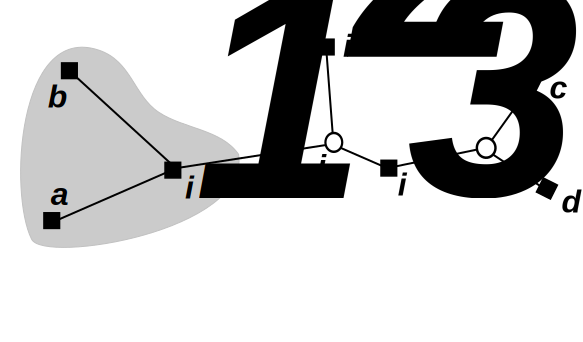
\includegraphics[height=1.6in]{objexp}
        \caption{A simple feasible solution illustrating the calculation of a contribution of node $i$ to the objective function. Destinations and Steiner nodes are denoted by solid squares and empty circles, respectively.}
                \label{fig:objexp}
\end{figure}

 The bjective function captures the entire network structure, and takes account of the  frequency of usage of certain power levels. In the example above, node $i$ uses the power level $p_{ii_2}$ every time the source of the relayed signal lies in the subtree $T_{i_1/i}$ which contains three potential sources. The power level $p_{ii_1}$ is used  whenever the source lies outside of $T_{i_1/i}$, which applies to four sources. The contribution of node $i$ to the objective function is thus $3p_{ii_2} + 4p_{ii_1}$. The total cost of $T$ is the sum over all nodes' contributions. In general, the total power consumption, or cost, is
$$
c(T) = \sum\limits_{i\in V_T}\left[nod(T_{i_1/i})p_{ii_2} + nod(T\setminus T_{i_1/i})p_{ii_1}\right].
$$ 
\begin{problem}\label{def:problem}
(SMT): Find a tree $T$ in $G$ such that $T$ spans $D$, and such that $c(T)$ is minimized.
\end{problem}
Like most of the wireless network design problems presented in the literature, SMT is NP-hard. This follows from the NP-hardness of SBT\cite{Papadimitriou06SBT}, which is the special case of Problem \ref{def:problem} where $D=V$.

\section{MILP Formulations Based on Broadcast Trees}
\label{sec:ILP}

In this section, we state and explain MILP formulations of the SMT problem. A basic element of every MIP formulation for SMT is a set of constraints modelling a Steiner tree. We investigate two such Steiner tree models with variables of up to 3 node indices and compare SMT models based on them. Both models are subsequently strengthened by valid inequalities. Introducing variables with 4 node indices and relevant constraints further extends the models. Valid inequalities added to the extended models result in the strongest known SMT formulations.
\subsection{Original SMT Model [SMT-X1]}
The first model extends the SBT formulation \cite{Haugland12Dual} by the Steiner nodes in order to formulate the multicast version of the problem. 
\subsubsection{Formulation}
Define the binary variables
\newline\newline
  $z_{ij}=
	\begin{cases}
    1 & \text{if edge $\{i,j\} \in E$ is in the solution},\\
    0 & \text{otherwise},
  \end{cases}$
\newline\newline
  $x^{s}_{ij}=
	\begin{cases}
    1 & \text{if arc $(i,j) \in A$ is used to transmit a message from $s\in D$},\\
    0 & \text{otherwise}.
  \end{cases}$
  \newline\newline
  $y^s_{ij}=
	\begin{cases}
    1 & \text{if node $i \in V$ uses power $p_{ij}$ to transmit a message from $s\in D$},\\
    0 & \text{otherwise}.
  \end{cases}$
\newline
\newline    
The following text often uses vectors $x^s=(x^s_{ij})_{(i,j)\in A}$  and $y^s=(y^s_{ij})_{(i,j)\in A}$ for each $s\in D$. The model SMT-X1 is formulated as:
\begin{subequations}\label{eq:smt-x1}
\begin{flalign}
\label{objective:dd} &\makebox[0pt][l]{$\displaystyle{}\min \sum\limits_{(i,j) \in A} \sum\limits_{s \in D} p_{ij} y^s_{ij} $}  & &&\\ \notag  
\text{s.t.}&  &  &                 && \\	\
%\label{con:dd:maxsize}\sum\limits_{\{i,j\}\in E}z_{ij} & \leq  N-1 &  && \\
\label{con:dd:arrowFromDest} \sum\limits_{j\in V_i}x^s_{ji} & = 1 && i,s\in D,i\neq s && \\ 
\label{con:dd:arrowFromNonDestB} \sum\limits_{j\in V_{i}}x^s_{ji} & \leq 1 && i\in V \setminus D, s\in D   &&\\	
\label{con:dd:arrowFromNonDestA} x^s_{ij}  & \leq \sum\limits_{k\in V_{i}\setminus \{j\}}x^s_{ki} && i\in V \setminus D,(i,j)\in A, s\in D   &&\\	
\label{con:dd:oneDir} x^s_{ij} + x^s_{ji} & = z_{ij} && \{i,j\}\in E, s\in D &&\\
\label{con:dd:startInSource}  x^s_{js}    & = 0   &&  s\in D, (j,s)\in A &&\\		 
\label{con:dd:yvar} x^s_{ij} & \leq \sum\limits_{k\in V:p_{ik}\geq p_{ij}}y^s_{ik} && s\in D, (i,j)\in A &&\\  
& \label{con:dd:vardim}	\mathbf{z} \in \{0,1\}^{E}, \mathbf{x},\mathbf{y}\in \{0,1\}^{A\times D} &&	
\end{flalign}~
\end{subequations}  
This model is slightly improved SMT model introduced in \cite{ivanova16isco} which contains a weaker version of constraint (\ref{con:dd:arrowFromNonDestA}).  
Let $(x,y,z)$ be an optimal solution to SMT-X1. Then, $x^s\in \{0,1\}^{A}$ induces a broadcast Steiner arborescence $H$ rooted at the source $s\in D$. From $z\in \{0,1\}^E$ we obtain the resulting (undirected) broadcast Steiner tree. Finally, $y^s\in \{0,1\}^{A}$ describes the links determining the power levels used by the nodes when relaying a message originated in $s$. The graph induced by $y$ is  a subgraph of the tree induced by $x$, and is not necessarily connected.

Constraints (\ref{con:dd:arrowFromDest})-(\ref{con:dd:startInSource}) model a Steiner tree. Constraint (\ref{con:dd:arrowFromDest}) ensure that a message from source $s$ reaches a destination $i$ from exactly one neighbour $j\in V_i$. Analogously, (\ref{con:dd:arrowFromNonDestB}) covers the case when $i \in V\setminus D$: for every source $s$, there is at most one inbound arc to a non-destination $i$. 

If a non-destination $i$ forwards a message from $s$ towards $j$, it receives the same message from a neighbour $k$ different from $j$. This is enforced by (\ref{con:dd:arrowFromNonDestA}). 
%Note that assuming there is no outgoing arc from a non-destination $j$, (\ref{con:dd:arrowFromNonDestA}) does not prevent $j$ from being a leaf in $G_{\mathbf{x^s}}$. Even though such solutions do not change the objective value of an integral solution, a Steiner tree by definition does not contain Steiner leaves.  We therefore disallow them by adding constraint (\ref{con:dd:extraCon}) reducing the set of feasible solutions. 

Expression (\ref{con:dd:oneDir}) enforces that an edge $\{i,j\}$ is part of a solution if and only if for every $s\in D$, either $(i,j)$ or $(i,j)$ is an arc used for sending a message from $s$. The next constraint (\ref{con:dd:startInSource}) expresses that a transmission initiated by $s\in D$ cannot reach $s$ again, which implies non-existence of a directed cycle containing $s$. 

Finally, by (\ref{con:dd:yvar}), we define a relation between $x$-variables and $y$-variables used in the objective function. Whenever the arc $(i,j)$ is used for transmission of a message from $s\in D$, the power assigned to node $i$ must be at least $p_{ij}$.
\subsubsection{Valid inequalities [SMT-X1-VI]}

It is possible to strengthen SMT-X1 by adding the valid inequalities
  \begin{subequations}[resume]
  \begin{flalign}
  \label{con:dd:extraCon} \sum\limits_{j\in V_{i}}x^s_{ji} & \leq \sum\limits_{j\in V_{i}}x^s_{ij}  \quad\quad ~~  	i\in V\setminus D, s\in D \\	
 \label{con:vi:Y1}  \sum\limits_{j\in V_s}  y^{s}_{sj} & =1,  \quad\quad\quad\quad\quad s\in D \\
\label{con:vi:sumYImpSumX} \sum\limits_{j\in V_i }y^{s}_{ij} & \geq \sum\limits_{j\in V_i}  x^{s}_{ji},  ~ \quad\quad   i\in V\setminus D, s\in D 
\end{flalign}
  \end{subequations}
Constraint (\ref{con:dd:extraCon}) ensures that $G_{x^s}$, and also any feasible solution, does not contain Steiner leaves. Even though the presence of Steiner leaves does not increase the objective value of an integral solution, it is desirable to eliminate them, because by definition, a Steiner tree does not contain non-destination leaves. Inequality (\ref{con:vi:Y1}) says that there has to be exactly one neighbour $j\in V$ of $s\in D$, such that $s$ uses the power $p_{sj}$ in order to transmit its own signal. A signal never disappears in a non-destination. As (\ref{con:vi:sumYImpSumX}) states, if a non-destination $i$ receives a signal from $s$, then there is a node $j\in V$ to which the signal is forwarded requiring power $p_{ij}$ assigned to node $i$.

\subsection{Multi-flow Extension [SMT-X2]}
This section shows how to use a network flow in order to strengthen the model further.
\subsubsection{Formulation}
\label{sec:smtx2:form}
Consider a multi-commodity network flow problem where one unit of commodity $(s,t)$ must be sent from $s\in D$ to $t\in D$. For this purpose, let $S=\{(s,t)\in D\times D, s\neq t\}$ be the set of ordered pairs of distinct destinations. In order to model the connectivity requirements, we introduce a variable $f^{st}_{ij}$ as follows:
\newline\newline
  $f_{ij}^{st}=
	\begin{cases}
    1 & \text{if arc $(i,j) \in A$ carries 1 unit of flow from $s$ to $t$, $(s,t)\in S$},\\
    0 & \text{otherwise}.
  \end{cases}$
\newline\newline
The relation between the $x$-variables in SMT-X1 and the $f$-variables is easy to see. If an arc $(i,j)$ carries a flow from $s$ to $t$, then $(i,j)$ is used for transmitting a signal initiated by $s$.
SMT-X1 can be strengthened by flow conservation constraints for each $(s,t)$-pair, which gives 
\newline
\newline    
\begin{subequations}\label{eq:smt-x2}
\begin{flalign}
\label{objective:dd} \makebox[0pt][l]{$\displaystyle{} \min \sum\limits_{(i,j) \in A} \sum\limits_{s \in D} p_{ij} y^s_{ij} $}  \\ 
\text{s.t.}    \notag   \\	
(\ref{con:dd:arrowFromDest}) - (\ref{con:dd:yvar}), (\ref{con:vi:Y1}), (\ref{con:vi:sumYImpSumX}) \notag \\ 
 \label{con:mf:flowNormal}  \sum\limits_{\substack{ j\in V_i}}f^{st}_{ij}-\sum\limits_{\substack{j\in V_i }}f^{st}_{ji}    & = 0   \quad \quad\quad 			  (s,t)\in S, i\in V\setminus\{s,t\} &\\	
\label{con:mf:flowDest}  \sum\limits_{\substack{ j\in V_t }}f^{st}_{tj}-\sum\limits_{\substack{j\in V_t}}f^{st}_{jt}    & = -1  \quad\quad ~ (s,t)\in S &\\	
 \label{con:mf:fcap}   f^{st}_{ij} &\leq  x^{s}_{ij},\quad\quad    (i,j)\in A, (s,t)\in S & \\ 		 			 	 
 \label{con:mf:fsym}   f^{st}_{ij} &=  f^{ts}_{ji},  \quad\quad(i,j)\in A, (s,t)\in S &\\   
\label{con:mf:xydim}	\mathbf{z} \in \{0,1\}^{E}, \mathbf{x},\mathbf{y} &\in \{0,1\}^{A\times D},  \mathbf{f}\in\{0,1\}^{A\times S}. 
\end{flalign}~
\end{subequations}  
The flow conservation constraints (\ref{con:mf:flowNormal})-(\ref{con:mf:flowDest}) guarantee that for each $(s,t)\in S$, one unit of commodity $(s,t)$ flows from $s$ to $t$. Next, constraint (\ref{con:mf:fcap}) expresses that if an arc $(i,j)$ carries an $s,t$-flow , then this arc is used for sending a message initiated in $s$. The flow symmetry (\ref{con:mf:fsym}) states that arc $(i,j)$ carries flow from $s$ to $t$ if and only if arc $(j,i)$ carries flow from $t$ to $s$.

\subsubsection{Valid inequalities [SMT-X2-VI]}

The flow variables introduced in Section \ref{sec:smtx2:form} suggest strengthening SMT-X2 by more valid inequalities involving these variables:

  \begin{subequations}[resume]
  \begin{flalign}
\label{con:vi:f2dest}  f^{st_1}_{ij}-f^{st_2}_{ij}+f^{t_1t_2}_{ij} & \geq 0, \quad\quad\quad\quad\quad\quad (i,j) \in A, \\  & \notag\quad\quad\quad\quad\quad\quad\quad\quad(s,t_1),(s,t_2),(t_1,t_2)\in S \\
\label{con:vi:xImpSumF} x^{s}_{ij} & \leq \sum\limits_{i\in V_j}  f^{st}_{ij},   \quad\quad   (i,j)\in A, (s,t)\in S \\
\label{con:vi:sumFImpSumY} \sum\limits_{i\in V_j, p_{ji}\geq p_{jk}  }f^{st}_{ji} & \leq \sum\limits_{i\in V_j, p_{ji}\geq p_{jk}}  y^{s}_{ji},   j,k\in V, (s,t)\in S.
\end{flalign}
  \end{subequations}
  
Assume $s,t_1,t_2\in D$. If there is flow via $(i,j)$ from $s$ to $t_2$, then $t_1$ lies either in $T_{i/j}$ or in $T_{j/i}$. In the former case, $(i,j)$ also carries a flow from $t_1$ to $t_2$. In the latter case, $(i,j)$ carries flow from $s$ to $t_1$. This is accomplished by (\ref{con:vi:f2dest}). By (\ref{con:vi:xImpSumF}) we state that whenever an arc $(i,j)$ carries a signal from $s$, there is at least one destination other than $s$ receiving it. That means that $(i,j)$ carries an $(s,t)$-flow from $s$ to $t$.  Consider nodes $j,k\in V$ and a pair of destinations $(s,t)$. If an $(s,t)$-flow is sent through $(j,i)$ such that $p_{ji}\geq p_{jk}$, then a message from $s$ must be relayed by $j$ using power level at least $p_{jk}$. This is expressed by (\ref{con:vi:sumFImpSumY}).
\subsection{SMT based on F1 [SMT -F1]}

There are many formulations for the Steiner minimum tree problem, that can serve as a basis for modelling the SMT problem. We consider the formulation F1, a network flow based model studied in \cite{Polzin}, where the authors use abbreviation $P_{F}$. The model assumes a given $s_0\in D$ that plays a role of a unique source.  To simplify notation, let $D_0= D_{s_0}$.
\subsubsection{Formulation}
Model F1 for the minimum Steiner tree problem contains variables
%\newline
%  $y^s_{ij}=
%	\begin{cases}
%    1 & \text{if node $i \in V$ uses power $p_{ij}$ to transmit messages from $s\in D$},\\
%    0 & \text{otherwise}.
%  \end{cases}
\newline\newline  
  $f^{t}_{ij}=
	\begin{cases}
    1 & \text{if arc $(i,j) \in A$ carries flow from $v_0$ to $t\in D_0$},\\
    0 & \text{otherwise},
  \end{cases}$  
\newline\newline  
  $x_{ij}=
	\begin{cases}
    1 & \text{if arc $(i,j) \in A$ is in the solution},\\
    0 & \text{otherwise}.
  \end{cases}$  
\newline
\newline   
The $x$-variables inducing the resulting tree correspond to arcs, and analogous $z$-variables in the SMT-X1 model correspond to edges. Hence, an optimal solution to SMT-X1 is an undirected tree, whereas optimal solutions to F1 are arborescences rooted at $s_0$. The vector $f^t$ defines a directed path from $s_0$ to $t\in D$ in the arborescence.

We aim to create the model SMT-F1 based on F1 from \cite{Polzin}. For this purpose, it is necessary to find a way to represent the constraint (\ref{con:dd:yvar}) in the F1 space. The $y$-variables from SMT-X1 have to be used in the extended F1, because they appear in the objective function which remains unchanged. By considering the role of individual sets of variables in both models, the $x$-variables used in SMT-X1 are expressed by the variables used SMT-F1 as
\begin{align}
\label{eq:tr:xijsB}x^s_{ij}&= x_{ij}-f^s_{ij} + f^{s}_{ji} & (i,j)\in A, s\in D_0
\end{align}


%The following equations express the transformations from PF2 to SMTMF space.
%\begin{subequations}
%\begin{align}
%\notag\label{eq:tr:fstij}f^{st}_{ij}&=f^t_{ij}(1-\check{f}^{st}_{ij})+f^{s}_{ji}(1-\check{f}^{st}_{ji})= \\
%&=  f^t_{ij}+f^s_{ji} - \check{f}^{st}_{ij} - \check{f}^{st}_{ji}& (i,j)\in A, \{s,t\}\in S_0\\
%\notag\label{eq:tr:xijj}x^s_{ij}&=x_{ij}(1-f^{s}_{ij})(1-f^{s}_{ji})+x_{ji}f^{s}_{ji}=
%\\&= x_{ij}-f^s_{ij} + f^{s}_{ji} & (i,j)\in A, s\in D_0\\
%\label{eq:tr:zij}z_{ij}&=x_{ij}+x_{ji}& \{i,j\}\in E
%\end{align}
%\end{subequations}
Let $(f,x,y)$ be an optimal solution to an SMT instance. Then
%By a similar approach, we achieve the transformation from SMTMF space to PF2 space. 
%\begin{subequations}
%\begin{align}
%\label{eq:tr:fstij2}x_{ij}=&x^0_{ij} & (i,j)\in A\\
%\label{eq:tr:fijt2}f^t_{ij}=&x^t_{ji}x^0_{ij}=f^{0t}_{ij} & (i,j)\in A, t\in D_0\\
%\label{eq:tr:fstij2}\check{f}^{st}_{ij}=& x^s_{ji}x^t_{ji}x^0_{ij} & (i,j)\in A, \{s,t\}\in S_0
%\end{align}
%\end{subequations}

%Let $T=(V_T,E_T)$ be a multicast tree, and consider an edge $\{i,j\}\in E_T$ dividing $T$ into two subtrees $T_i$ and $T_j$ rooted in $i$ and $j$, respectively.  If the arc $(i,j)$ is used for sending a message from $s\in D$ to $t\in D$, then $s$ and $t$ must lie in different subtrees. Node $v_0$ lies either in $T_i$ or $T_j$, as depicted in Fig. \ref{fig:transf_a} and Fig. \ref{fig:transf_b}, respectively. These two cases are captured by the first equality in (\ref{eq:tr:fstij}). If both $v_0$ and $s$ lie in $T_i$, then $f_{ij}^t=1$. Similarly, if $v_0$ and $t$ lie in $T_j$, then $f_{ji}^s=1$. The expressions in parentheses prevent $s$ and $t$ belonging to the same subtree. Further, using the implications $\check{f^{st}_{ij}}=1\Rightarrow f_{ij}^t=1$ and $\check{f^{st}_{ji}}=1\Rightarrow f_{ji}^s=1$ that follow from the interpretation of variables, we justify the second equality expressing this relation linearly.
%\begin{figure*}[h!]
%    \centering
%    \begin{subfigure}[b]{0.5\textwidth}
%       \centering
%       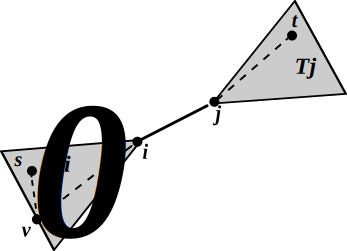
\includegraphics[height=1.2in]{transf_a}
%        \caption{}
%       \label{fig:transf_a}
%   \end{subfigure}%
%    \begin{subfigure}[b]{0.5\textwidth}
%        \centering
%        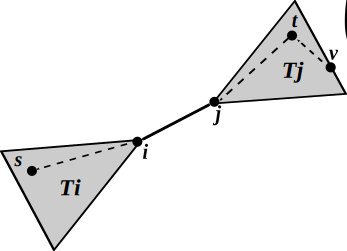
\includegraphics[height=1.2in]{transf_b}
%        \caption{}
%                \label{fig:transf_b}
%    \end{subfigure}
%    \caption{Explanation of the transformations (\ref{eq:tr:fstij}) - (\ref{eq:tr:zij})}
%    \label{fig:transexp}
%\end{figure*}

%In the transformation (\ref{eq:tr:xijj}) of $x_{ij}^s$, we distinguish the situation when $v_0$ and $s$ are in the same subtree, in which case none of the arcs $(i,j)$ and $(j,i)$ carries a flow to $s$, and when $s$ and $v_0$ belong to different subtrees, and there is a flow via $(j,i)$ towards $s$. Again, the last equality is justified since $f_{ij}^s=1\Rightarrow x_{ij}=1$. The relation (\ref{eq:tr:zij}) is obvious.

Having this transformation in hand, it is easy to construct a SMT-F1 model based on the minimum Steiner tree model F1:

    \begin{subequations}
    \begin{flalign}
  \min &  \sum\limits_{(i,j) \in A} \sum\limits_{s \in D} p_{ij} y^s_{ij}    \\  \notag  
		   \text{s.t.}&                  && \\	\ 
\label{con:pf1:xfrel}  f^{t}_{ij}   &\leq x_{ij}    ~~ \qquad \qquad t\in D_0, (i,j)\in A \\
 \label{con:pf1:flow}  \sum\limits_{\substack{ j \in V_i }}f^{t}_{ji}-\sum\limits_{\substack{j\in V_i}}f^{t}_{ij}    & = \begin{cases}
    1~~~~&  t\in D_0, t = i \\        0~~~~ \qquad             & t\in D_0, i\in V\setminus \{s_0, t\}\end{cases}     \\	
%\label{con:pf2:flowSource}  \sum\limits_{\substack{ j \in V_i }}\check{f}^{st}_{ji}-\sum\limits_{\substack{j\in V_i}}\check{f}^{st}_{ij}    & \geq \begin{cases}
%    -1~~~&  \{s,t\}\in S_0, i = v_0 \\        0  ~~~~   \qquad    & \{s,t\}\in S_0, i\in V\setminus \{v_0\}\end{cases}     \\			
%\label{con:pf2:hookImpFs}  \check{f}^{st}_{ij}    & \leq f^s_{ij}~~   \qquad  \qquad \{s,t\}\in S_0, (i,j)\in A \\	
%\label{con:pf2:hookImpFt}  \check{f}^{st}_{ij}    & \leq f^t_{ij}~~   \qquad    \qquad \{s,t\}\in S_0, (i,j)\in A \\			 		
% \label{con:pf2:stronger}  f^{s}_{ij}+f^{t}_{ij}-\check{f}^{st}_{ij}    &\leq x_{ij}    ~~ \qquad \qquad  \{s,t\}\in S_0, (i,j)\in A \\			 
 \label{con:pf1:flowX}  \sum\limits_{\substack{ j\in V_i }}x_{ji}-\sum\limits_{\substack{j\in V_i}}x_{ij}    & \leq 0~~~~    \qquad\qquad			  i\in V\setminus D \\			 			   	
\label{con:pf1:yvar} x_{ij} -f^t_{ij}+f^t_{ji}  &\leq \sum\limits_{\substack{k\in V: \\ p_{ik}\geq p_{ij}}}y^t_{ik}   ~~\quad  t\in D_0, (i,j)\in A \\  		
\label{con:pf1:yvar0} x_{ij} &\leq \sum\limits_{\substack{k\in V: \\ p_{ik}\geq p_{ij}}}y^0_{ik}   ~~\quad  (i,j)\in A \\  		
\label{con:pf1:B}  \sum_{j\in V_i}x_{ji}&\leq 1~~~~ \qquad  \qquad i\in V\setminus D\\
\label{con:pf1:noflowFromT} f_{ti}^t&=0 ~~~~ \qquad  \qquad t\in D_0, i\in V_t   \\
\label{con:pf1:fitt=xit} f_{it}^t&=x_{it} ~~ \qquad  \qquad t\in D_0, i\in V_t \\
\label{con:pf1:xi0=0} x_{i0}&=0 ~~~~ \qquad  \qquad i\in V_0 \\
%\label{con:pf1:fi0s=0} f_{i0}^t&=0 ~~~~ \qquad  \qquad i\in V_0, t\in D_0 \\
%\label{con:pf1:fij0=0} f_{ij}^0&=0 ~~~~ \qquad  \qquad (i,j)\in A \\	   			  
\label{con:pf1:dim}	\mathbf{x} \in \{0,1\}^{A},\mathbf{f}&\in\{0,1\}^{A \times D} \\ 
\label{con:pf1:dimy} \mathbf{y}&\in \{0,1\}^{A\times D}
    \end{flalign}~
    \end{subequations}
    
    Constraints (\ref{con:pf1:xfrel})-(\ref{con:pf1:flow}) together with (\ref{con:pf1:dim}) imply that $\mathbf{x}$ induces and arborescence spanning $D$ with node $v_0$ as the root. The constraint (\ref{con:pf1:yvar}) has the same purpose as (\ref{con:dd:yvar}), and is expressed in SMT-F1 space using transformation (\ref{eq:tr:xijsB}). Note that the $y_{ij}^s$-variables determining power levels are defined for all destinations $s\in D$, while in the F1 model of the minimum Steiner tree problem, the $f_{ij}^s$ variables are defined only for $s\in D_0$. 
%This inconsistency is resolved by adding (\ref{con:pf1:yvar0}), which relates the $y^0$-variables with $x$-variables. This is equivalent to extending the the domain of the $f$-variables and fixing the newly introduced variables to zero. 
\begin{figure}[!htb]
    \centering
    \begin{subfigure}[b]{0.4\textwidth}
        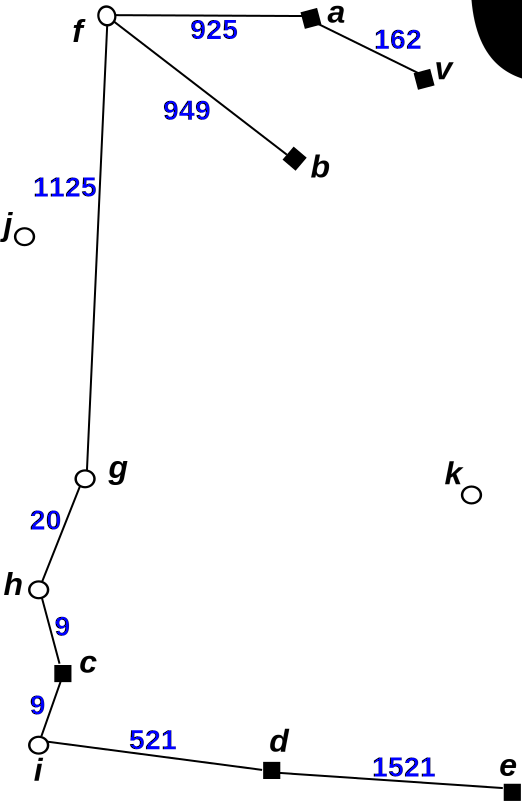
\includegraphics[width=\textwidth]{conBNec}
        \caption{Optimal solution obtained by SMT-X1. The $z$-variables inducing the resulting tree in this model represent undirected edges. The objective value of this tree is 25156.}
        \label{fig:BorigSMT}
    \end{subfigure}
    \hfill %add desired spacing between images, e. g. ~, \quad, \qquad, \hfill etc. 
      %(or a blank line to force the subfigure onto a new line)
    \begin{subfigure}[b]{0.4\textwidth}
        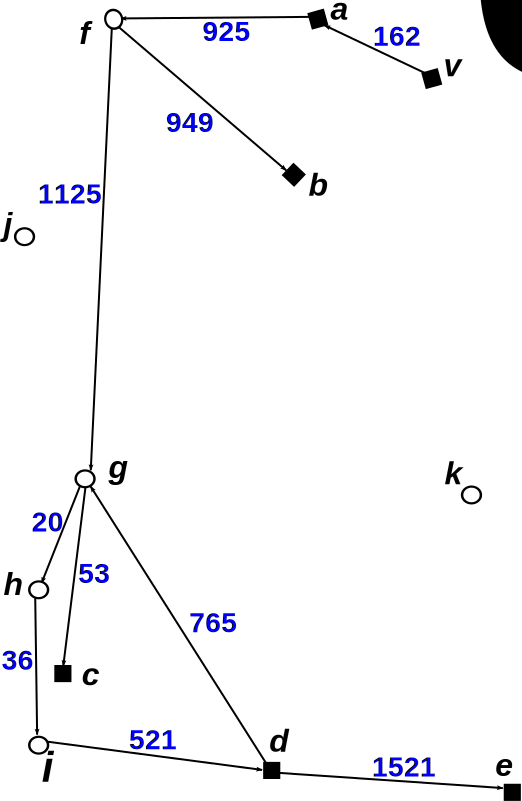
\includegraphics[width=\textwidth]{conBNec2}
        \caption{Solution obtained by SMT-F1 without constraint \ref{con:pf1:B} with objective value 25148. The nodes are connected by arrows because the tree yielded by this model is rooted in a predefined source $v_0$.}
        \label{fig:Bpf2}
    \end{subfigure}
    \caption{An exemplary instance showing why the constraint (\ref{con:pf1:B}) is necessary in SMT-F1. Blue numbers denote power requuirements of connection between nodes. For better legibility, the distances of the links are not proportional.} \label{fig:BProof}
\end{figure}   
     By (\ref{con:pf1:B}) we prevent a non-destination from having multiple entering arcs. This is not necessary in the minimum Steiner tree problem formulation F1, because the objective function causes that such solutions are filtered out by optimality. The necessity of this constraint in SMT is demonstrated in Fig. \ref{fig:BProof}. The optimal solution with objective value 25156 to the depicted instance obtained by solving SMT-X1 is shown in Fig. \ref{fig:BorigSMT}. The solution in Fig \ref{fig:Bpf2} yielded by solving SMT-F1 without the constraint (\ref{con:pf1:B}) has objective value 25148, but is not a feasible solution to Problem \ref{def:problem}, because of the cycle $(g,h,i,d,g)$. The non-existence of such a cycle in a solution given by model SMT-X1 is ensured by constraints (\ref{con:dd:arrowFromDest}), (\ref{con:dd:arrowFromNonDestB}) and (\ref{con:dd:oneDir}). A detailed proof of this claim can be found in \cite{ivanova16isco}. A transmission commenced in node $c$ is sent via arc $(g,f)$. As a consequence of the link between $g$ and $d$ in Fig. \ref{fig:Bpf2}, the node $d$ also receives the message. This link is absent in Fig. \ref{fig:BorigSMT}, and so $i$ has to relay the signal using the arc $(i,d)$, causing the higher total objective value. Similarly, the obviously valid inequalities (\ref{con:pf1:noflowFromT})-(\ref{con:pf1:xi0=0}) are not necessary in the minimum Steiner tree formulation, but have to be included included in the formulation of SMT, because they  disallow nodes in $D_0$ having multiple entering arcs. The same restriction has to be imposed on $v_0$ by adding (\ref{con:pf1:xi0=0}).
   
\begin{prop}
\label{prop:modelcorrect}
If $(\mathbf{f},\mathbf{x})$ satisfies (\ref{con:pf1:flow}) - (\ref{con:pf1:flowX}) and (\ref{con:pf1:B})-(\ref{con:pf1:dim}) then $G_{x}$ is an arborescence spanning $D$ rooted at $v_0$.
\end{prop}
 
 \begin{proof}
 The connectivity of $G_\mathbf{x}$ as well as coverage of all nodes from $D$ is ensured by flow constraints (\ref{con:pf1:flow}) and relation (\ref{con:pf1:xfrel}). The absence of both directed and undirected cycles is enforced by (\ref{con:pf1:B})-(\ref{con:pf1:xi0=0}). These constraints together imply that no node has more than one entering arc. Solutions, where nodes from $V\setminus D$ are leaves are excluded due to (\ref{con:pf1:flowX}).\qed
 \end{proof}
 
\subsubsection{Valid inequalities [SMT-F1-VI]}
The same valid inequalities as in SMT-X1-VI can be added to SMT-F1, leading to the SMT-F1-VI model. Inequality (\ref{con:vi:Y1}) can be added without any change. The $x$-variable in (\ref{con:vi:sumYImpSumX}) has to be replaced by the equivalent expression defined by (\ref{eq:tr:xijsB}) which gives
\begin{subequations}[resume]
\begin{flalign}
\label{con:vi:sumYImpSumXTrans} \sum\limits_{j\in V_i }y^{s}_{ij} & \geq \sum\limits_{j\in V_i}  \left(x_{ji}-f^s_{ji}+f^s_{ij}\right).   \quad\quad   i\in V\setminus D, s\in D 
\end{flalign}
\end{subequations}
\subsection{F2 Extension [SMT-F2]}
Similarly to the extension SMT-X2 of SMT-X1 by the $s-t$-flow variables, the SMT-F1 model can also be extended by variables with four node indices. Analogously to $S$, let $\check{S}=\{\{s,t\}\subseteq D: s\neq t\}$ be the set of unordered pairs of destinations, and let $\check{S}_0=\{\{s,t\}\in S: s\neq v_0\neq t\}$. 
\subsubsection{Formulation}
The authors of \cite{Polzin} use variables
\newline\newline  
  $\check{f}^{st}_{ij}=
	\begin{cases}
    1 & \text{if arc $(i,j) \in A$ carries flow from $v_0$ to both $s$ and $t$, $\{s,t\}\in \check{S}_0$},\\
    0 & \text{otherwise},
  \end{cases}$
  \newline\newline  
  describing a common flow from $v_0$ to $s$ and $t$. This allows formulation of an extended model, SMT-F2: 
    \begin{subequations}
    \begin{flalign}
  \min &  \sum\limits_{(i,j) \in A} \sum\limits_{s \in D} p_{ij} y^s_{ij}    \\  \notag  
		   \text{s.t.}&                  && \\			   
		   (\ref{con:pf1:xfrel}) - (\ref{con:pf1:xi0=0}), (\ref{con:vi:Y1}),(\ref{con:vi:sumYImpSumXTrans}) \notag \\ 	
\label{con:pf2:flowHook}  \sum\limits_{\substack{ j \in V_i }}\check{f}^{st}_{ji}-\sum\limits_{\substack{j\in V_i}}\check{f}^{st}_{ij}    & \geq \begin{cases}
    -1~~~&  \{s,t\}\in \check{S_0}, i = 0 \\        0  ~~~~   \qquad         & \{s,t\}\in \check{S_0}, i\in V\setminus \{v_0\}\end{cases}     \\			
\label{con:pf2:startInSource}  \check{f}^{st}_{ij}    & \leq f^s_{ij}~~   \qquad  \qquad \{s,t\}\in \check{S_0}, (i,j)\in A \\	
\label{con:pf2:stopInDest}  \check{f}^{st}_{ij}    & \leq f^t_{ij}~~   \qquad    \qquad \{s,t\}\in \check{S_0}, (i,j)\in A \\			 		
 \label{con:pf2:stronger}  f^{s}_{ij}+f^{t}_{ij}-\check{f}^{st}_{ij}    &\leq x_{ij}    ~~ \qquad \qquad  \{s,t\}\in \check{S_0}, (i,j)\in A \\			 	   			  
 \label{con:pf2:dim}  \mathbf{x}     \in \{0,1\}^A,  \mathbf{f}&\in \{0,1\}^{A\times D}, \mathbf{\check{f}}\in\{0,1\}^{A\times \check{S}}\\
 \label{con:pf2:dim2}  \mathbf{y} & \in \{0,1\}^{A\times D}
    \end{flalign}~
    \end{subequations}

By (\ref{con:pf2:flowHook}) is ensured that the common flow is non-increasing. The inequalities (\ref{con:pf2:stronger}) replace a weaker (\ref{con:pf1:xfrel}). It follows from the domain of $\check{f}$, that 
\begin{equation}
\label{eq:fhooksym}
\check{f}_{ij}^{st}=\check{f}_{ij}^{ts},
\end{equation}
because $S_0$ consists of unordered pairs. By the implicit assumption of (\ref{eq:fhooksym}) in SMT-F2, it is possible to infer additional valid inequalities for SMT. We can also write
\begin{align*}
\check{f}^{st}_{ij}+\check{f}^{st}_{ji}=\check{f}^{ts}_{ij}+\check{f}^{ts}_{ji} &\Rightarrow f^t_{ij}+f^s_{ji}-f^{st}_{ij}=f^s_{ij}+f^t_{ji}-f^{ts}_{ij}\Rightarrow \\ & \Rightarrow f^{0t}_{ij}+f^{0s}_{ji}-f^{st}_{ij}=f^{0s}_{ij}+f^{0t}_{ji}-f^{ts}_{ij}.
\end{align*}
The first and second implication follow from the transformation (\ref{eq:tr:fstij}) and (\ref{eq:tr:fijt2}), respectively. The last equality consists of only variables from SMT-X2  space, and so the valid inequality
\begin{equation*}f^{ut}_{ij}+f^{us}_{ji}+f^{ts}_{ij}=f^{us}_{ij}+f^{ut}_{ji}+f^{st}_{ij} \quad\quad (u,t),(u,s),(s,t),(t,s)\in S_0, i,j\in V
\end{equation*} 
can be added to  SMT-X2. All the occurances of $v_0$ were replaced by a general destination $u\in D$, because $v_0$ does not have any special role in SMT-X2.

\subsubsection{Valid inequalities [SMT-F2-VI]}

To complete the listing of models, we state the SMT-F2-VI model created by adding transformed valid inequalities (\ref{con:vi:f2dest})-(\ref{con:vi:sumFImpSumY}) to SMT-F2 :

\section{Relations Between the Models}
\label{sec:comp}
In order to create the SMT-F1 model, it is necessary to express $x^s_{ij}$ variables in F1 space using relation (\ref{eq:tr:xijsB}). The aim of this section is to show how the entire SMT-X2 model can be converted into an equivalent model that uses only variables of SMT-F2. 

The following equations express all variables from SMT-X2 in SMT-F2 space:
\begin{subequations}
\begin{align}
\notag\label{eq:tr:fstij}f^{st}_{ij}&=f^t_{ij}(1-\check{f}^{st}_{ij})+f^{s}_{ji}(1-\check{f}^{st}_{ji})= \\
&=  f^t_{ij}+f^s_{ji} - \check{f}^{st}_{ij} - \check{f}^{st}_{ji}& (i,j)\in A, \{s,t\}\in S_0\\
\notag\label{eq:tr:xijj}x^s_{ij}&=x_{ij}(1-f^{s}_{ij})(1-f^{s}_{ji})+x_{ji}f^{s}_{ji}=
\\&= x_{ij}-f^s_{ij} + f^{s}_{ji} & (i,j)\in A, s\in D_0\\
\label{eq:tr:zij}z_{ij}&=x_{ij}+x_{ji}& \{i,j\}\in E
\end{align}
\end{subequations}

Let $T=(V_T,E_T)$ be a tree covering $D$, and consider an edge $\{i,j\}\in E_T$ dividing $T$ into two subtrees $T_i$ and $T_j$ rooted in $i$ and $j$, respectively.  If the arc $(i,j)$ caries and $s-t$-flow from $s\in D$ to $t\in D$, then $s$ and $t$ must lie in different subtrees. Node $v_0$ lies either in $T_i$ or $T_j$.
%as depicted in Fig. \ref{fig:transf_a} and Fig. \ref{fig:transf_b}, respectively.
These two cases are captured by the first equality in (\ref{eq:tr:fstij}). If both $v_0$ and $s$ lie in $T_i$, then $f_{ij}^t=1$. Similarly, if $v_0$ and $t$ lie in $T_j$, then $f_{ji}^s=1$. The expressions in parentheses prevent $s$ and $t$ belonging to the same subtree. Using the implications $\check{f^{st}_{ij}}=1\Rightarrow f_{ij}^t=1$ and $\check{f^{st}_{ji}}=1\Rightarrow f_{ji}^s=1$ that follow from the interpretation of variables, we justify the second equality expressing this relation linearly.
%\begin{figure*}[h!]
%    \centering
%    \begin{subfigure}[b]{0.5\textwidth}
%       \centering
%      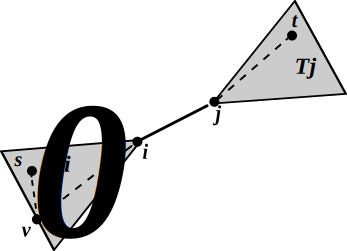
\includegraphics[height=1.2in]{transf_a}
%        \caption{}
%       \label{fig:transf_a}
%   \end{subfigure}%
%    \begin{subfigure}[b]{0.5\textwidth}
%        \centering
%        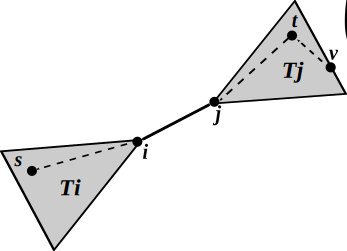
\includegraphics[height=1.2in]{transf_b}
%        \caption{}                \label{fig:transf_b}
%    \end{subfigure}
%    \caption{Explanation of the transformations (\ref{eq:tr:fstij}) - (\ref{eq:tr:zij})}
%    \label{fig:transexp}
%\end{figure*}
In the transformation (\ref{eq:tr:xijj}) of $x_{ij}^s$, we distinguish the situation when $v_0$ and $s$ are in the same subtree, in which case none of the arcs $(i,j)$ and $(j,i)$ carries a flow to $s$, and when $s$ and $v_0$ belong to different subtrees, and there is a flow via $(j,i)$ towards $s$. Again, the last equality is justified since $f_{ij}^s=1\Rightarrow x_{ij}=1$. The relation (\ref{eq:tr:zij}) is obvious.

By a similar approach, we achieve the transformation from SMT-X2 space to SMT-F2 space. 
\begin{subequations}
\begin{align}
\label{eq:tr:fstij2}x_{ij}=&x^0_{ij} & (i,j)\in A\\
\label{eq:tr:fijt2}f^t_{ij}=&x^t_{ji}x^0_{ij}=f^{0t}_{ij} & (i,j)\in A, t\in D_0\\
\label{eq:tr:fstij2}\check{f}^{st}_{ij}=& x^s_{ji}x^t_{ji}x^0_{ij} & (i,j)\in A, \{s,t\}\in \check{S}_0
\end{align}
\end{subequations}

We aim to compare the models presented in Section \ref{sec:ILP} in terms of strength. The results obtained by numerical experiments presented in the next section suggest, that SMT-F1-VI model is stronger than SMT-X2. This section proves this conjecture. 
First, we express the SMT-X2 model in SMT-F2 space using transformations (\ref{eq:tr:fstij})-(\ref{eq:tr:zij}). 
%This formulation is referred to as MF-PF2.
 %	\begin{small} 	
\begin{subequations}
\begin{flalign}
\label{objective:mfinpf2} &\makebox[0pt][l]{$\displaystyle{}\min \sum\limits_{(i,j) \in A} \sum\limits_{s \in D} p_{ij} y^s_{ij} $}  & &&\\ \notag  
   \text{s.t.}&  &  &                 && \\	\
%\label{con:mfinpf2:maxsize}   \sum\limits_{\{i,j\}\in E}(x_{ij}+x_{ji}) & \leq  N-1  &   && \\
     \label{con:mfinpf2:arrowFromDest}  \sum\limits_{j\in V_i}(x_{ji}-f^s_{ji}+f^s_{ij})          & = 1       			&& i\in D, s\in D_0, i \neq s && \\ 
		  \label{con:mfinpf2:arrowFromNonDestB}  \sum\limits_{j \in V_i}(x_{ji}-f^s_{ji}+f^s_{ij})  &\leq 1 && i\in V \setminus D, s\in D_0   &&\\		
		  \label{con:mfinpf2:arrowFromNonDestA}  x_{ij}-f^s_{ij}+f^s_{ji}  & \leq \sum\limits_{k \in V_i\setminus\{j\}}(x_{ki}-f^s_{ki}+f^s_{ik}) &&
		  i\in V \setminus D,j\in V_i, s\in D_0   &&\\		  
      \label{con:mfinpf2:extraCon}  \sum\limits_{j \in V_i}(x_{ji}-f^s_{ji}+f^s_{ij}) & \leq \sum_{\mathclap{j \in V_i}}(x_{ij}-f^s_{ij}+f^s_{ji}) &&  i\in V\setminus D, s\in D_0  &&\\			  \label{con:mfinpf2:startInSource}  x_{js} - f^s_{js}+f^s_{sj}    & = 0       			&&  s\in D_0, j\in V_s &&\\		 
		  \label{con:mfinpf2:yvar}  x_{ij}-f^s_{ij}+f^s_{ji} & \leq \sum\limits_{k\in V:p_{ik}\geq p_{ij}}y^s_{ik} && s\in D, (i,j)\in A 		&&\\  
		  \label{con:mfinpf2:yvar0} x_{ij} &\leq \sum\limits_{\substack{k\in V: \\ p_{ik}\geq p_{ij}}}y^0_{ik}   && (i,j)\in A \\  		
		 		 \label{con:mfinpf2:flowNormal}  \sum\limits_{\substack{ j\in V_i }}f^t_{ij}-\sum\limits_{\substack{j\in V_i }}f^t_{ji}    & = 0     			&& i\in V, t\in D_0, i \neq t &&\\	
		 	 \label{con:mfinpf2:flowDest}  \sum\limits_{\substack{j\in V_t}}f^t_{tj}-\sum\limits_{\substack{j\in V_t}}f^t_{jt}    & = -1     			&&  t \in D_0 &&\\	
%		 			 	 \label{con:mfinpf2:flowSource}  \sum\limits_{\substack{ (s,j)\in A}}(f^t_{sj}+f^s_{js})-\sum\limits_{\substack{(j,s)\in A}}(f^t_{js}+f^s_{sj})    & = 1     			&&  \{s,t\}\subseteq D_0 && \\	
           \label{con:mfinpf2:fcap}   f^t_{ij} - \check{f}^{st}_{ij} - \check{f}^{st}_{ji} &\leq  x_{ij}-f^s_{ij}   && (i,j)\in A, \{s,t\}\in \check{S}_0 && &\\ 		 			 	 
		    \label{con:mfinpf2:zbound} x_{ij}+x_{ji}&\leq 1 &&\{i,j\}\in E \\
  		    \label{con:mfinpf2:xbound} 0&\leq x_{ij}-f_{ij}^s+f_{ji}^s  \leq 1 && \{i,j\}\in E,  s\in D_0 \\
\label{con:mfinpf2:fbound} 0&\leq f_{ij}^t+f_{ji}^s-\check{f}_{ij}^{st}-\check{f}_{ji}^{st}  \leq 1 && \{i,j\}\in E,\{s,t\}\in \check{S}_0 \\
%(\ref{con:pf1:xi0=0}) - (\ref{con:pf1:fij0=0}) \notag \\ 
		    \label{con:mfinpf2:dim}	\mathbf{x} \in \{0,1\}^{A},\mathbf{f}&\in\{0,1\}^{A \times D},\mathbf{\check{f}}\in\{0,1\}^{A\times \check{S}} \\ 
		    \label{con:mfinpf2:dimy}\mathbf{y}&\in \{0,1\}^{A\times D}
    \end{flalign}
    \end{subequations}  
%\end{small}

Note that the 4-index variables $\check{f}^{st}_{ij}$ appear only in (\ref{con:mfinpf2:fcap}) and (\ref{con:mfinpf2:fbound}). Assigning the highest possible values $\check{f}^{st}_{ij}=f^{t}_{ij}$ and $\check{f}^{st}_{ji}=f^{s}_{ji}$ according to (\ref{con:mfinpf2:fbound}) does not cause a violation of any other constraint. In this case (\ref{con:mfinpf2:fcap}) becomes the same as the first inequality in (\ref{con:mfinpf2:xbound}). It is therefore possible to remove (\ref{con:mfinpf2:fcap}) and (\ref{con:mfinpf2:fbound}), resulting in a model in SMT-F1 space (with up to 3-index variables) equivalent to the SMT-X2 model. The following lemmas are useful for the analysis of the relations between the models. 
\begin{lemma}
All solutions satisfying LP(SMT-F1-VI) satisfy
\begin{align*}
\sum_{j\in V_i}x_{ji}&=1,~~~~~~ i\in D_0. & \label{eq:sumToD} \tag{A}\\
%f_{ij}^t&\leq x_{ij},~~~~ (i,j)\in A, t\in D_0. & \label{eq:fimpx} \tag{B} \\
\end{align*}
\end{lemma}
\begin{proof}
 Utilizing first (\ref{con:pf1:fitt=xit}), next (\ref{con:pf1:flow}) for $t=i$, and finally (\ref{con:pf1:noflowFromT}), we get
$$\sum_{j\in V_i}x_{ji}=\sum_{j\in V_i}f_{ji}^i = 1+\sum_{j\in V_i}f_{ij}^i=1.$$\qed
\end{proof}
\begin{lemma}\label{lem:onedir} For any SMT instance, there exists an optimal solution to model LP(SMT-F1-VI) such that
$\forall (i,j)\in A, t\in D_0: \min\{f_{ij}^t,f_{ji}^t\} = 0.$
\end{lemma}
\begin{proof}
Assume that $\exists t\in D_0: \min\{f_{ij}^t,f_{ji}^t\} = \epsilon> 0$ in an optimal solution. It is then possible to reduce the flow towards $t$ along the cycle $(i,j,i)$ by $\epsilon$. Flow conservation remains satisfied because for both $i$ and $j$, entering and leaving flow towards $t$ is reduced by the same amount. All remaining constraints are satisfied and the objective value is not altered because 
$$
x_{ij}-(f_{ij}^t-\epsilon)+(f_{ji}^t-\epsilon) = x_{ij}-f_{ij}^t+f_{ji}^t.
$$
Such a solution is therefore an alternative optimal solution satisfying the property stated by this lemma.  \qed
\end{proof}
In the following text, let $f^*_{ij}=\max_{t\in D_0}\{f^t_{ij}\}$.
\begin{lemma}\label{lem:oneslack} For any SMT instance, there exists an optimal solution to model LP(SMT-F1-VI) such that 
%$\forall i,j\in V: x_{ij} = f^*_{ij} \vee x_{ji}=f^*_{ji}$.
$\forall (i,j)\in A: \min\{x_{ij} - f^*_{ij}, x_{ji}-f^*_{ji}\}=0$.
\end{lemma}
\begin{proof}
If $\exists (i,j)\in A: \min\{x_{ij} - f^*_{ij}, x_{ji}-f^*_{ji}\}=\epsilon>0$, it would be possible to decrease both $x_{ij}$ and $x_{ji}$ by $\epsilon$ which does not increase the objective value and does not violate any constraint. In particular, the lhs in (\ref{con:pf1:flowX}) remains unchanged after this operation.  \qed
\end{proof}
\begin{lemma}\label{lem:xequals} Let $(f,x,y)$ be an optimal solution to an SMT instance. Then for each arc $(i,j)\in A$, at least one of the following properties holds:

\begin{itemize}
\item\label{lem:item:noslack} $x_{ij}=f^*_{ij},$\hfill(L.\ref{lem:xequals}a)
%\item\label{lem:item:slack} $\sum_{k\in V_i}x_{ki} - \sum_{k\in V_i\setminus\{j\}} x_{ik} - f^*_{ij} > 0, $ and (\ref{con:pf1:flowX}) is satisfied with equality.
\item\label{lem:item:slack} %$x_{ij} > f^*_{ij}$ and 
(\ref{con:pf1:flowX}) is satisfied with equality.\hfill(L.\ref{lem:xequals}b)
\end{itemize}

\end{lemma}
\begin{proof}
First we realize that by decreasing $x_{ij}$, the objective value can not increase. This variable can be reduced as long as it preserves feasibility of the solution. The only constraints that could be violated by reducing $x_{ij}$ are (\ref{con:pf1:xfrel}) and (\ref{con:pf1:flowX}), and so assigning 
$$x_{ij}\coloneqq\max\bigg\{ f^*_{ij},\sum_{k\in V_i}x_{ki}-\sum_{k\in V_i\setminus\{j\}}x_{ik}\bigg\}$$
either does not change the value $x_{ij}$, or yields an alternative optimum. \qed
\end{proof}
For clarification of the case \ref{lem:item:slack}), consider an instance with a feasible solution depicted in Fig. \ref{fig:counterex}.
\begin{figure}[h!]
        \centering
        \includegraphics[height=2.3in]{counterex}
        \caption{A feasible solution to LP(SMT-F1-VI) of an instance on six vertices. Labels of the edges are values of $f$-vectors. Blue numbers represent $f^{t_1}$ components, red numbers correspond to $f^{t_2}$ components.} 
                \label{fig:counterex}
\end{figure}
In this solution, the case \ref{lem:item:noslack}) fails for the edge $\{b,c\}$, because if $x_{s_0b}=x_{ab}=0.5$, then $x_{bc}$ must be equal to 1 in order to fulfill (\ref{con:pf1:flowX}). This situation can occur only when two different flows join at some non-destination node and then continue via a shared edge. The flows must be different, because if they were towards the same destination, the size of the flow via the shared edge would be equal to their sum and so the case \ref{lem:item:noslack}) would not be violated. In our example the two different flows are aiming to $t_1$ and $t_2$, they join at $b$, and then continue together through $(b,c)$.


\begin{prop}
\label{prop:f1strx2}
LP(SMT-F1-VI) is at least as strong as LP(SMT-X2). 
\end{prop}
\begin{proof}
We analyze whether all solutions satisfying LP(SMT-F1-VI) satisfy LP(SMT-X-F). This is done by showing that each inequality in LP(SMT-F1-VI) is implied by inequalities in LP(SMT-X-F) 

\begin{itemize}
%\item[] (\ref{con:mfinpf2:maxsize}): Folaws directly from (\ref{eq:sumToD}) and (\ref{con:pf1:B}).
\item[] (\ref{con:mfinpf2:arrowFromDest}): Assume $t\in D_0$ and $i\in D_0\setminus\{t\}$. Flow conservation (\ref{con:pf1:flow}) implies
$$\sum_{j\in V_i}x_{ji} - \sum_{j\in V_i}f_{ji}^t + \sum_{j\in V_i}f_{ij}^t = \sum_{j\in V_i}x_{ji}.$$ Then (\ref{con:mfinpf2:arrowFromDest}) follows from (\ref{eq:sumToD}).
Assume $i=v_0$: Due to (\ref{con:pf1:xi0=0}) and (\ref{con:pf1:xfrel}), the first two sums equal to zero, which gives
$$\sum_{j\in V_i}x_{ji} - \sum_{j\in V_i}f_{ji}^t + \sum_{j\in V_i}f_{ij}^t = \sum_{j\in V_i}f_{ij}^t = 1,$$
where the latter equality follows by summing (\ref{con:pf1:flow}) over all $i\in V\setminus\{v_0\}$.
\item[] (\ref{con:mfinpf2:arrowFromNonDestB}): The proof is analogous to (\ref{con:mfinpf2:arrowFromDest}), with (\ref{con:pf1:B}) replacing (\ref{eq:sumToD}).
\item[] (\ref{con:mfinpf2:arrowFromNonDestA}): The inequality can be rewritten as
\begin{align*}
 x_{ij}  \leq& \sum\limits_{k \in V_i\setminus\{j\}}x_{ki}-\sum\limits_{k \in V_i\setminus\{j\}}f^s_{ki}+\sum\limits_{k \in V_i\setminus\{j\}}f^s_{ik} +f^s_{ij}-f^s_{ji} = \\
 ~=& \sum\limits_{k \in V_i\setminus\{j\}}x_{ki}-\sum\limits_{k \in V_i}f^s_{ki}+\sum\limits_{k \in V_i}f^s_{ik} = \sum\limits_{k \in V_i\setminus\{j\}}x_{ki},
\end{align*}
where the last equality follows from the flow conservation (\ref{con:pf1:flow}). Now assume the contrary that
\begin{align}
x_{ij} > \sum\limits_{k \in V_i\setminus\{j\}}x_{ki}.\label{eq:assumContr}\tag{B}
\end{align}
The proof is divided into two parts that capture the two cases stated by Lemma \ref{lem:xequals}. If option (L.4a) holds, we have that $\exists t\in D_0 \text{ s. t. }f^t_{ij}=x_{ij}$.
It follows from Lemma \ref{lem:onedir} that $f^t_{ji}=0$, and by utilizing (\ref{con:pf1:xfrel}) we get
$$f^t_{ij}=x_{ij}>\sum\limits_{k \in V_i\setminus\{j\}}x_{ki} \geq \sum\limits_{k \in V_i\setminus\{j\}}f^t_{ki}=\sum\limits_{k \in V_i}f^t_{ki},$$
which contradicts flow conservation constraints (\ref{con:pf1:flow}).
In case option (L.4b) applies, we know from Lemma \ref{lem:oneslack} that $x_{ji}=f^*_{ji}$, and so $\exists t\in D_0 \text{ s. t. }f^t_{ji}=x_{ji}$. Moreover, Lemma \ref{lem:onedir} says that if for some $s\in D_0: f^s_{ji}>0$, then $f^s_{ij} = 0$, i.e. any flow that enters $i$ via $(ji)$ must leave it through an arc different from $(ij)$. Together with the flow conservation and (\ref{con:pf1:xfrel}),
$$
x_{ji}=f^t_{ji}\leq\sum_{k\in V_i}f^t_{ik}=\sum_{k\in V_i\setminus\{j\}}f^t_{ik}\leq\sum_{k\in V_i\setminus\{j\}}x_{ik}.
$$
Note that for $x_{ji}=f^t_{ji}=0$, $f^t_{ij}\geq 0$ in which case the equality would not hold, but we could directly write $x_{ji}\leq\sum_{k\in V_i\setminus\{j\}}x_{ik}$. Combined with the assumption \ref{eq:assumContr} we obtain
$$
\sum_{k\in V_i}x_{ki} = x_{ji} + \sum_{k\in V_i\setminus\{j\}}x_{ki}<x_{ij} + \sum_{k\in V_i\setminus\{j\}}x_{ik} = \sum_{k\in V_i}x_{ik},
$$
which is in contradiction with (L.4b) that asserts that (\ref{con:pf1:flowX}) is satisfied with equality. We have shown that every possibility that assumes that the negation of (\ref{con:mfinpf2:arrowFromNonDestA}) holds leads to a contradiction, and thereby finalized the proof of (\ref{con:mfinpf2:arrowFromNonDestA}).
\item[] (\ref{con:mfinpf2:extraCon}): Follows immediately from (\ref{con:pf1:flowX}) by utilizing flow conservation (\ref{con:pf1:flow}) at node $j$.
\item[] (\ref{con:mfinpf2:startInSource}): Follows from (\ref{con:pf1:noflowFromT}) and (\ref{con:pf1:fitt=xit}).
\item[] (\ref{con:mfinpf2:yvar}): Follows from (\ref{con:pf1:yvar}).
\item[] (\ref{con:mfinpf2:flowNormal})-(\ref{con:mfinpf2:flowDest}): All four-index variables cancel out. Thus, (\ref{con:mfinpf2:flowNormal}) follows from flow conservation (\ref{con:pf1:flow}) at $i$.
%\item[] (\ref{con:mfinpf2:fcap}): Follows from (\ref{con:pf2:stronger}).
\item[] (\ref{con:mfinpf2:zbound}): %First, let us consider the case \ref{lem:item:noslack}) in Lemma \ref{lem:xequals}, where $\exists t\in D_0$ such that $f^t_{ij}=x_{ij}$. Assume for contradiction that $x_{ij}+x_{ji}>1$ for some $\{i,j\}\in E$.  By the flow conservation, $\sum_{k\in V_{i}}f^t_{ki}\geq f^t_{ij}=x_{ij}.$ Also, from Lemma \ref{lem:onedir} we know that $f^t_{ji}=0$, and so we can write 
%\[
%1< x_{ij}+x_{ji}\leq\sum_{k\in V_{i}}f^t_{ki}+x_{ji}\leq\smashoperator{\sum_{k\in V_{i}\setminus\{j\}}}f^t_{ki}+x_{ji}\leq\smashoperator{\sum_{k\in V_{i}\setminus\{j\}}}x_{ki}+x_{ji}=\sum_{k\in V_{i}}x_{ki},
%\]
%$$\sum_{k\in V_{i}\setminus\{j\}}f^t_{ki}+x_{ji}>1\Rightarrow\sum_{k\in V_{i}\setminus\{j\}}x_{ki}+x_{ji}>1\Rightarrow\sum_{k\in V_{i}}x_{ki}>1,$$
%contradicting either (\ref{eq:sumToD}), if $i\in D_0$, or (\ref{con:pf1:B}), if $i\in V\setminus D$. Now let us assume %that $f^*_{ij}<x_{ij}$ and
% (\ref{con:pf1:flowX}) is satisfied with equality.
 Adding $x_{ji}$ to both sides of (\ref{con:mfinpf2:arrowFromNonDestA}) gives the desired relation
\[
x_{ij}+x_{ji}\leq\sum_{k\in V_i\setminus\{j\}}x_{ki} +x_{ji}=\sum_{k\in V_i}x_{ki}\leq 1,
\]
Where the last inequality follows from (\ref{con:pf1:B}) if $i\in V\setminus D$, and is replaced by equality due to (\ref{eq:sumToD}) in case $i\in D$.
%It is sufficient to show this case for a non-destination $i$, because for $i\in D$,  $x_{ij}=f^*_{ij}$ would certainly hold, which is covered by the previous case. 
\item[] (\ref{con:mfinpf2:xbound}): The lower bound follows from (\ref{con:pf1:xfrel}). The upper bound follows from (\ref{con:mfinpf2:arrowFromDest}) for $i\in D$ and from (\ref{con:mfinpf2:arrowFromNonDestB}) for $i\in V\setminus D$. To see this, observe that each term in the sums in (\ref{con:mfinpf2:arrowFromDest})-(\ref{con:mfinpf2:arrowFromNonDestB}) is non-negative because of (\ref{con:pf1:xfrel}). 
%\item[] (\ref{con:mfinpf2:fbound}): The lower bound follows from (\ref{con:pf2:hookImpFs})-(\ref{con:pf2:hookImpFt}). From (\ref{eq:fimpx}) and (\ref{con:mfinpf2:zbound}), we get the upper bound
$$f^t_{ij}+f^s_{ji}-f^{st}_{ij}-f^{st}_{ji}\leq f^t_{ij}+f^s_{ji}\leq x_{ij}+x_{ji}\leq 1$$
\end{itemize}\qed
\end{proof} 
Note that in parts (\ref{con:mfinpf2:arrowFromNonDestA}) and (\ref{con:mfinpf2:xbound}) of this proof it is necessary to assume SMT-F1 instead of SMT-F2. The arguments work with (\ref{con:pf1:xfrel}), but could not be used with stronger (\ref{con:pf2:stronger}).
Proposition \ref{prop:f1strx2} suggests that additional 4-index variables in SMT-X2 model are not very useful, because the formulation is implied by the smaller SMT-F1-VI. However, SMT-X2 is justified because of valid inequalities (\ref{con:vi:f2dest})-(\ref{con:vi:sumFImpSumY}) that significantly strengthen the model and can also be converted into SMT-F2 space and also increased the LP bound.

%From (\ref{con:pf2:hookImpFs}), (\ref{con:pf2:hookImpFt}) and (\ref{eq:tr:fijt2}) we have that $\check{f}^{st}_{ij}\leq f^{0s}_{ij}$ and $\check{f}^{st}_{ij}\leq f^{0t}_{ij}$. Combining these two inequalities yields valid inequalities
%\[
%\left.
%\begin{array}{ll}
%\check{f}^{st}_{ij}+\check{f}^{st}_{ji}&\leq f^{0s}_{ij}+f^{0s}_{ji} \\[.2cm]
%check{f}^{st}_{ij}+\check{f}^{st}_{ji}&\leq f^{0s}_{ij}+f^{0t}_{ji} \\[.2cm]
%\check{f}^{st}_{ij}+\check{f}^{st}_{ji}&\leq f^{0t}_{ij}+f^{0s}_{ji} \\[.2cm]
%\check{f}^{st}_{ij}+\check{f}^{st}_{ji}&\leq f^{0t}_{ij}+f^{0t}_{ji} 
%\end{array}
%\right\} \Rightarrow
%\left\{
%\begin{array}{ll}
%f^{st}_{ij}&\geq f^{0t}_{ij}-f^{0s}_{ij} \\[.2cm]
%f^{st}_{ij}&\geq f^{0t}_{ij}-f^{0s}_{ij} + f^{0s}_{ji} - f^{0t}_{ji} \\[.2cm]
%f^{st}_{ij}&\geq 0 \\[.2cm]
%f^{st}_{ij}&\geq f^{0s}_{ji}-f^{0t}_{ji}
%\end{array}.
%\right.
%\]
%If some of them are not already implied by constraints in SMTMF, the can be included in the model. The implication is justified by (\ref{eq:tr:fstij}) and (\ref{eq:tr:fijt2}).

\section{Constraint Generation}
\label{sec:cg}
The stronger models SMT-X2-VI and SMT-F2-VI are too large and are therefore not very practical for solving even fairly small instances.  The main idea of how to make this model more useful in practice is to solve a relaxation of the model where some of the constraints are omitted. Relaxed constraints that are violated in the obtained solutions can be dynamically added to the model and the whole process is repeated, until some termination criteria are fulfilled. This approach is known as a \emph{constraint generation scheme}.

\subsection{SMT-X2-VI}%
First, the constraint generation scheme is applied to SMT-X2-VI. We relax the flow constraints, which means that we solve only LP(SMT-X1). This gives the vector $\mathbf{x}$ that, according to constraint (\ref{con:mf:fcap}), acts as a capacity vector, and determines the maximum possible amount of flow through certain arc. We then go through all possible $s-t$ pairs of destinations and check whether the flow constraints are fulfilled for the particular $s$ and $t$. This is equivalent to solving a maximum flow problem, and those $s-t$-pairs for which there is no feasible solution are stored. When all pairs are processed, new flow constraints for some (possibly all) stored $s-t$-pairs are added to the model, and the whole process is repeated until there are no violated flow constraints for any $s-t$ pair. The algorithm \ref{alg:congen} describes this process more formally.

There are various strategies how to determine which of the violated flow constraints will be added to the model. 


\section{Experimental Evaluation}
\label{sec:exp}

The practical part of this work focuses on comparison of the models presented in the previous section. As the main focus of this study is to determine tighter bounds, the conducted experiments are designed for this purpose. Instances of intended number of vertices are generated with random coordinates uniformly distributed between [0, 0] and [100, 100]. All computations were made on an Intel Core 2 Quad CPU at 2.83 GHz and 8 GB RAM.

\subsection{Instance generation}


\subsection{Comparison of the models}
\label{sec:conclusion}
In the following experiments, two different scenarios are considered. First, we create instances with constant number of destinations, and the number of non-destinations gradually increases. Conversely, in the second scenario, the number of non-destinations is fixed, while the number of destinations increases. The models are compared with respect to the objective value of their solutions and CPU time.

We compared models LP(SMT-X1), SMTMF-LP, SMTPF2-LP and SMT-X1, with results marked in graphs in Fig. \ref{fig:id-basi}. We can clearly see that the SMTMF-LP and SMTPF2-LP are stronger than LP(SMT-X1), and the difference increases with increasing number of nodes. Nevertheless, the best LP bounds are still far from the integer solution. The difference between SMTMF-LP and SMTPF2-LP seems negligible, however, the latter one is always slightly stronger, in average by 0.33\% for the largest instances. 

The CPU time of the SMTPF2-LP model seems to be more favourable than SMTMF-LP for instances with lower ratio $|V|/|D|$. 
%\begin{figure*}[h!]
%    \centering
%    \begin{subfigure}[b]{0.5\textwidth}
%        \centering
%        \includegraphics[height=1.2in]{../graphs/id-basic-cost}
%        \caption{}
%        \label{fig:id-basic-cost}
%    \end{subfigure}%
 %   \begin{subfigure}[b]{0.5\textwidth}
 %       \centering
%        \includegraphics[height=1.2in]{../graphs/id-basic-time}
%        \caption{}
%%                \label{fig:id-basic-time}
%    \end{subfigure}
%    \caption{}
%    \label{fig:id-basi}
%\end{figure*}


%\begin{figure*}[h!]
%    \centering
%    \begin{subfigure}[b]{0.5\textwidth}
%        \centering
%        \includegraphics[height=1.2in]{../graphs/in-basic-cost}
%        \caption{}
%        \label{fig:in-basic-cost}
 %   \end{subfigure}%
%    \begin{subfigure}[b]{0.5\textwidth}
%        \centering
%        \includegraphics[height=1.2in]{../graphs/in-basic-time}
%        \caption{}
                \label{fig:in-basic-time}
%    \end{subfigure}
%    \caption{}
%    \label{fig:in-basic}
%\end{figure*}

\section{Conclusion and Future Work}
\label{sec:conclusion}
%as required. Don't forget to give each section
%and subsection a unique label (see Sect.~\ref{sec:1}).
%\paragraph{Paragraph headings} Use paragraph headings as needed.
%\begin{equation}
%a^2+b^2=c^2
%\end{equation}

% For one-column wide figures use
%\begin{figure}
% Use the relevant command to insert your figure file.
% For example, with the graphicx package use
%  \includegraphics{example.eps}
% figure caption is below the figure
%\caption{Please write your figure caption here}
%\label{fig:1}       % Give a unique label
%\end{figure}
%
% For two-column wide figures use
%\begin{figure*}
% Use the relevant command to insert your figure file.
% For example, with the graphicx package use
%  \includegraphics[width=0.75\textwidth]{example.eps}
% figure caption is below the figure
%\caption{Please write your figure caption here}
%\label{fig:2}       % Give a unique label
%\end{figure*}
%
% For tables use
%\begin{table}
% table caption is above the table
%\caption{Please write your table caption here}
%\label{tab:1}       % Give a unique label
% For LaTeX tables use
%\begin{tabular}{lll}
%\hline\noalign{\smallskip}
%first & second & third  \\
%\noalign{\smallskip}\hline\noalign{\smallskip}
%number & number & number \\
%number & number & number \\
%\noalign{\smallskip}\hline
%\end{tabular}
%\end{table}


%\begin{acknowledgements}
%If you'd like to thank anyone, place your comments here
%and remove the percent signs.
%\end{acknowledgements}

% BibTeX users please use one of
%\bibliographystyle{spbasic}      % basic style, author-year citations
%\bibliographystyle{spmpsci}      % mathematics and physical sciences
%\bibliographystyle{spphys}       % APS-like style for physics
%\bibliography{}   % name your BibTeX data base

% Non-BibTeX users please use
\begin{thebibliography}{}
%
% and use \bibitem to create references. Consult the Instructions
% for authors for reference list style.
%
\bibitem{Wieseltier00onthe}
Wieselthier,  J. E., Nguyen, G. D., Ephremides, A.,
On the Construction of Energy-Efficient Broadcast and Multicast Trees in Wireless Networks,
Proceedings of the Nineteenth Annual Joint Conference of the IEEE Computer and Communications Societies.
2, 585--594 (2000)

\bibitem{Haugland12Dual}
Yuan, D., Haugland, D.,
Dual Decomposition for Computational Optimization of Minimum-Power Shared Broadcast Tree in Wireless Networks,
IEEE Transactions on Mobile Computing,
12, 11, 2008--2019 (2012)

\bibitem{Polzin}
Polzin, T., Daneshmand, S. V., A comparison of Steiner tree relaxations, Discrete Applied Mathematics, 112,  1-3, 15 241--261, (2001)

\bibitem{ivanova16isco}
Ivanova, M., Shared Multicast Trees in Ad Hoc Wireless Networks, Combinatorial Optimization, 4th International Symposium, ISCO 2016, 241--261, (2016)

\bibitem{Haugland11Compact}
Haugland, D., Yuan, D.,
Wireless Network Design: Optimization Models and Solution Procedure, 219--246,
International Series in Operations Research \& Management Science.
Springer, New York, (2011)

\bibitem{Papadimitriou06SBT}
Papadimitriou, I., and Georgiadis, L.:
Minimum-energy Broadcasting in Multi-hop Wireless Networks Using a Single Broadcast Tree.
Mobile Networks and Applications.
11, 3, 361--375 (2006)

%\bibitem{RefJ}
% Format for Journal Reference
%Author, Article title, Journal, Volume, page numbers (year)
% Format for books
%\bibitem{RefB}
%Author, Book title, page numbers. Publisher, place (year)
% etc
\end{thebibliography}

\end{document}
% end of file template.tex

